%%%%%%%%%%%%%%%%%%%%%%%%%%%%%%%%%%%%%%%%%%%%%%%%%%%%%%%%%%%%%%%%%%%%%%%%%%%%%%%%
% Template for USENIX papers.
%
% History:
%
% - TEMPLATE for Usenix papers, specifically to meet requirements of
%   USENIX '05. originally a template for producing IEEE-format
%   articles using LaTeX. written by Matthew Ward, CS Department,
%   Worcester Polytechnic Institute. adapted by David Beazley for his
%   excellent SWIG paper in Proceedings, Tcl 96. turned into a
%   smartass generic template by De Clarke, with thanks to both the
%   above pioneers. Use at your own risk. Complaints to /dev/null.
%   Make it two column with no page numbering, default is 10 point.
%
% - Munged by Fred Douglis <douglis@research.att.com> 10/97 to
%   separate the .sty file from the LaTeX source template, so that
%   people can more easily include the .sty file into an existing
%   document. Also changed to more closely follow the style guidelines
%   as represented by the Word sample file.
%
% - Note that since 2010, USENIX does not require endnotes. If you
%   want foot of page notes, don't include the endnotes package in the
%   usepackage command, below.
% - This version uses the latex2e styles, not the very ancient 2.09
%   stuff.
%
% - Updated July 2018: Text block size changed from 6.5" to 7"
%
% - Updated Dec 2018 for ATC'19:
%
%   * Revised text to pass HotCRP's auto-formatting check, with
%     hotcrp.settings.submission_form.body_font_size=10pt, and
%     hotcrp.settings.submission_form.line_height=12pt
%
%   * Switched from \endnote-s to \footnote-s to match Usenix's policy.
%
%   * \section* => \begin{abstract} ... \end{abstract}
%
%   * Make template self-contained in terms of bibtex entires, to allow
%     this file to be compiled. (And changing refs style to 'plain'.)
%
%   * Make template self-contained in terms of figures, to
%     allow this file to be compiled. 
%
%   * Added packages for hyperref, embedding fonts, and improving
%     appearance.
%   
%   * Removed outdated text.
%
%%%%%%%%%%%%%%%%%%%%%%%%%%%%%%%%%%%%%%%%%%%%%%%%%%%%%%%%%%%%%%%%%%%%%%%%%%%%%%%%

\documentclass[letterpaper,twocolumn,10pt]{article}
\usepackage{usenix2019_v3}

% to be able to draw some self-contained figs
\usepackage{tikz}
\usepackage{amsmath}

% inlined bib file
\usepackage{filecontents}

\usepackage{graphicx}
\usepackage{float}
\graphicspath{ {../images/}}

%-------------------------------------------------------------------------------
\begin{filecontents}{\jobname.bib}
%-------------------------------------------------------------------------------

\end{filecontents}

%-------------------------------------------------------------------------------
\begin{document}
%-------------------------------------------------------------------------------

%don't want date printed
\date{}

% make title bold and 14 pt font (Latex default is non-bold, 16 pt)
\title{\Large \bf The RISC Takers:\\
  Milestone Report I}

%for single author (just remove % characters)
\author{
  {\rm Sean Keever} \\
  swkeever@uw.edu
  \and
  {\rm Yokesh Jayakumar} \\
  mcmahjoh@uw.edu
  \and
  {\rm John McMahon} \\
  karthj@uw.edu
  % copy the following lines to add more authors
  % \and
  % {\rm Name}\\
  %Name Institution
} % end author

\maketitle

%-------------------------------------------------------------------------------
\begin{abstract}
  %-------------------------------------------------------------------------------
  The goal of our project is to create a means of letting a user not only use an OS,
  but to allow a user to see what is going on inside the OS and CPU.
  To this end, our project aims to maximize availability to users by
  providing a browser-based interface that lets the user visit a webpage and
  visualizing an OS from the moment he or she visits the page.
\end{abstract}

%-------------------------------------------------------------------------------
\section{Introduction}
%-------------------------------------------------------------------------------

There are multiple implementations of operating systems made available via a web
browser. Instead of re-implementing that functionality, we chose to find a project that
has the low-level emulation from C to JavaScript already handled. This way, we can
focus on solving a new problem: visualizing the OS and CPU.

We looked at multiple different OS implementations and decided on risv-angel,
which seemed to offer the
functionality we needed without too much underlying complexity. This way, we could
focus more attention to creating the visualization layers without having to worry
too much about the emulation implementation details.

%-------------------------------------------------------------------------------
\section{Initial Design}
%-------------------------------------------------------------------------------

To start, we stripped the riscv-angel project to only show the Terminal.
We got rid of all the elements and libraries that were not going to be used in our project.
Before we started on our implementation, we prototyped the UI in Figma, shown in \ref{fig:proto1}.

\begin{figure}[H]
  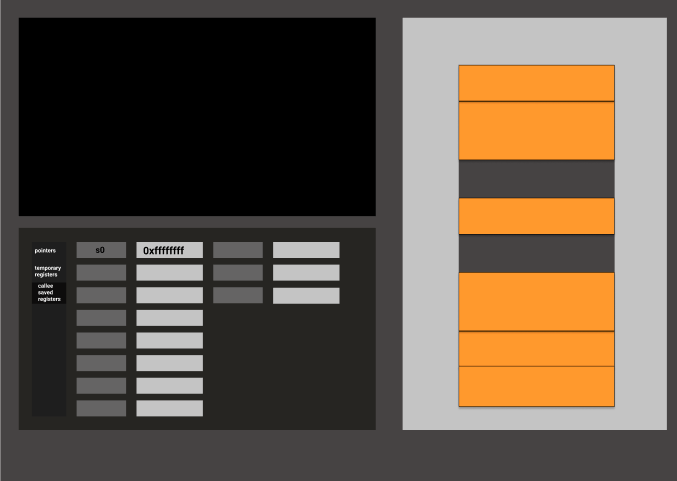
\includegraphics[scale=0.3]{prototype1}
  \caption{Initial prototype of design}
  \label{fig:proto1}
  \centering
\end{figure}

Figma allowed us to come up with a design before we implement anything in code.
We aimed for a dashboard-like interface, showing the user all the most important
information about the CPU and OS.
Right now, we know we want to show:

\begin{itemize}
  \item Contents of registers (show values of registers in real time)
  \item Contents of memory (let users zoom in on a particular region of memory)
\end{itemize}

\textbf{Question for the reader:} What else would be useful data to show to the user?
We are having some trouble figuring out what exactly would be useful data to show.
Also, we have memory data available to us, but of course, it is a \textit{lot} of data.
We are still determining what exactly we want to show in regards to memory.
Do you have any recommendations or opinions on this?

%-------------------------------------------------------------------------------
\section{Beginning Development}
%-------------------------------------------------------------------------------

\subsection*{Setting up a development environment}

One of the challenges for the team was facing ambiguity in this project.
It was difficult to interpret exactly what needed to be done.

To facilitate this problem and make development easier,
we started approaching the project with an Agile workflow.
We are using GitHub's Kanban board functionality to track issues and milestones.
We hold weekly stand-ups to find out

\begin{itemize}
  \item what we did over the past week, and
  \item what we will do in the next week.
\end{itemize}

\noindent
We use the GitHub issues that we created to assign tasks for each member of a group.
In doing this, we are hoping we can be more productive and have a more concrete
understanding of what needs to be done to complete the project.

To ensure robustness and quality of our project,
we have also developed some tooling for continuous integration.
To ensure consistency in the codebase, we use ESLint, a tool that we have configured
to apply the rules defined in AirBnB's style guide.

We also set up GitHub Actions, which are essentially hooks that execute when
code is pushed to the repository.
These hooks will run the style checker and our unit tests before code is pushed to remote.
The hook will reject any commits if any of these actions fail.

\subsection*{Choosing technologies}

We want our interface to be interactive, so we chose React.js as our library of choice,
which offers a means of rapidly developing interactive client-side applications.

This doesn't come without its challenges, though. The existing project uses vanilla JavaScript
in order to run the emulator. The legacy code accomplishes this by spawning a worker thread
that handles all the emulation tasks. The main thread interacts with this worker thread via
message passing.

This existing framework is most likely not going to work in our React app.
To use the existing code, we would
need to fetch the OS/CPU state via message passing. But we want our application to update in real
time as the user uses the OS. Thus, the only solution we see is polling the worker thread and
asking it for the most up-to-date view of CPU state. This strategy bogs down the application
and will not be a strategy that we can move forward with long term.

We will need to do work to port some of the legacy code into the React scope. This way, when
the OS is being used, React can know about the changes in state in real-time.
We think this refactor will increase performance substantially and will be necessary
if we want this application to be usable.


%-------------------------------------------------------------------------------
\section*{Future Plans}
%-------------------------------------------------------------------------------

By Milestone II, we aim to

\begin{itemize}
  \item finalize our UI prototype
  \item have all the base functionality of the application working
  \item start implementing the styling of the application
\end{itemize}

Then, in the time between Milestone II and the demo, we aim to

\begin{itemize}
  \item finish styling the application
  \item add bells and whistles to the application
  \item attempt to optimize performance, SEO, and possibly deploy the app.
\end{itemize}

\textbf{Question for the reader:} What do you think about these goals?
Are they too ambitious or not ambitious enough?
Do you have any suggestions or recommendations in general?

%-------------------------------------------------------------------------------
\section*{Acknowledgments}
%-------------------------------------------------------------------------------

Thanks to all of the contributors of \href{https://github.com/riscv/riscv-angel}{riscv-angel},
in which this project is based on.

%-------------------------------------------------------------------------------
\section*{Availability}
%-------------------------------------------------------------------------------

This project is open-source and is available at
\href{https://github.com/swkeever/riscv-angel-extended}
{https://github.com/swkeever/riscv-angel-extended}

%-------------------------------------------------------------------------------


%%%%%%%%%%%%%%%%%%%%%%%%%%%%%%%%%%%%%%%%%%%%%%%%%%%%%%%%%%%%%%%%%%%%%%%%%%%%%%%%
\end{document}
%%%%%%%%%%%%%%%%%%%%%%%%%%%%%%%%%%%%%%%%%%%%%%%%%%%%%%%%%%%%%%%%%%%%%%%%%%%%%%%%

%%  LocalWords:  endnotes includegraphics fread ptr nobj noindent
%%  LocalWords:  pdflatex acks
